\section{Đăng kí}


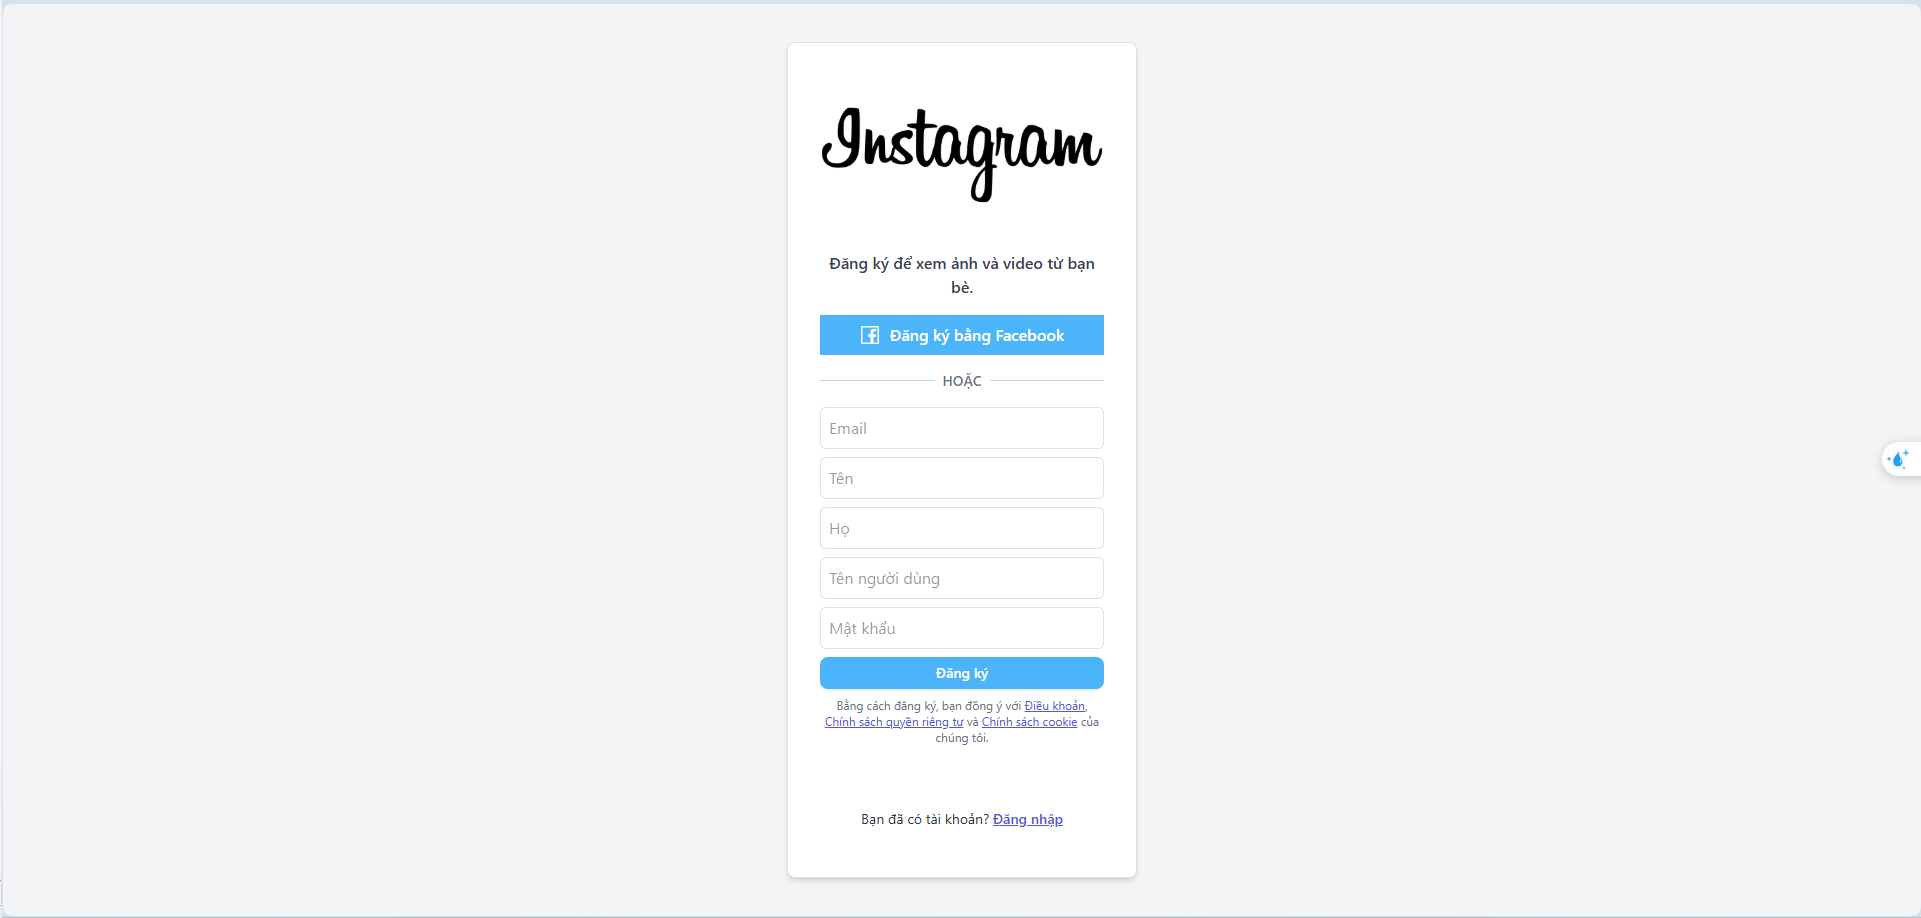
\includegraphics[width=1\textwidth]{img/instagram/dangki.png}
\begin{figure}[H]
    \centering
    \caption{Đăng kí}
\end{figure}


\FloatBarrier % <-- Dòng này sẽ khóa ảnh phía trên không bị dời xuống

\section{Đăng nhập}
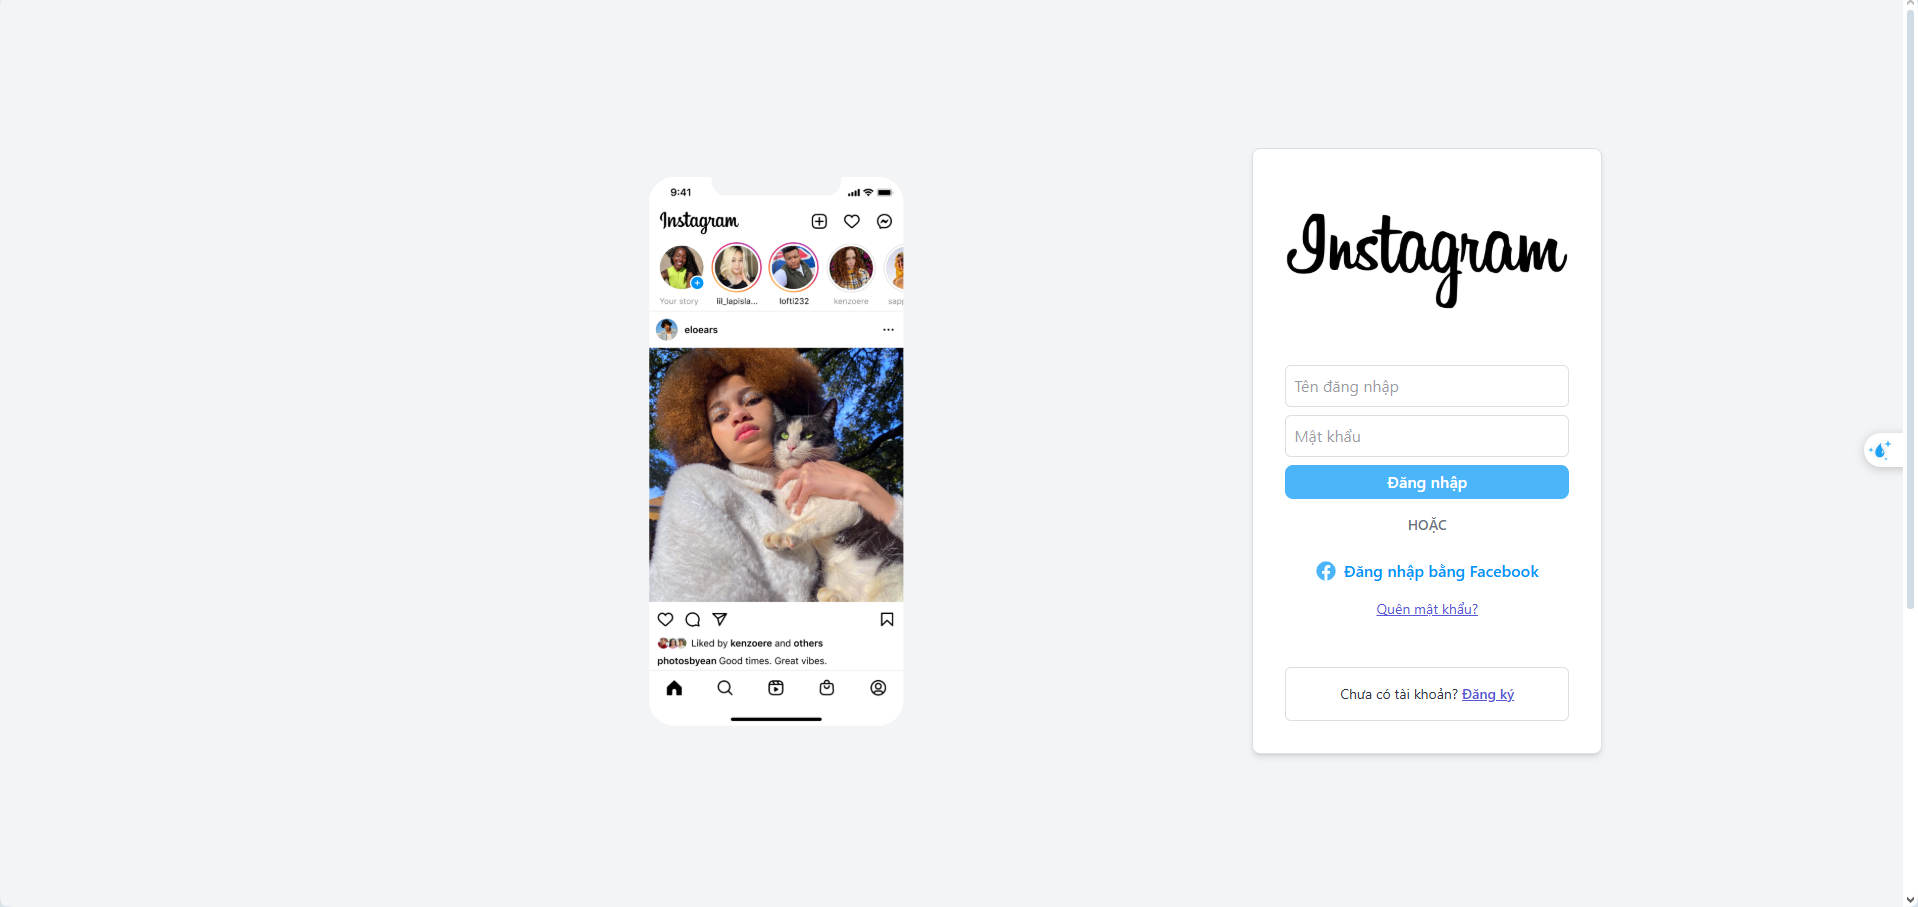
\includegraphics[width=1\textwidth]{img/instagram/dangnhap.png}
\begin{figure}[H]
    \centering
    \caption{Đăng nhập}
\end{figure}


\FloatBarrier % <-- Dòng này sẽ khóa ảnh phía trên không bị dời xuống


\section{Chức năng đăng bài viết}

\subsection{HÌnh ảnh}

\begin{figure}[H]
    \centering
    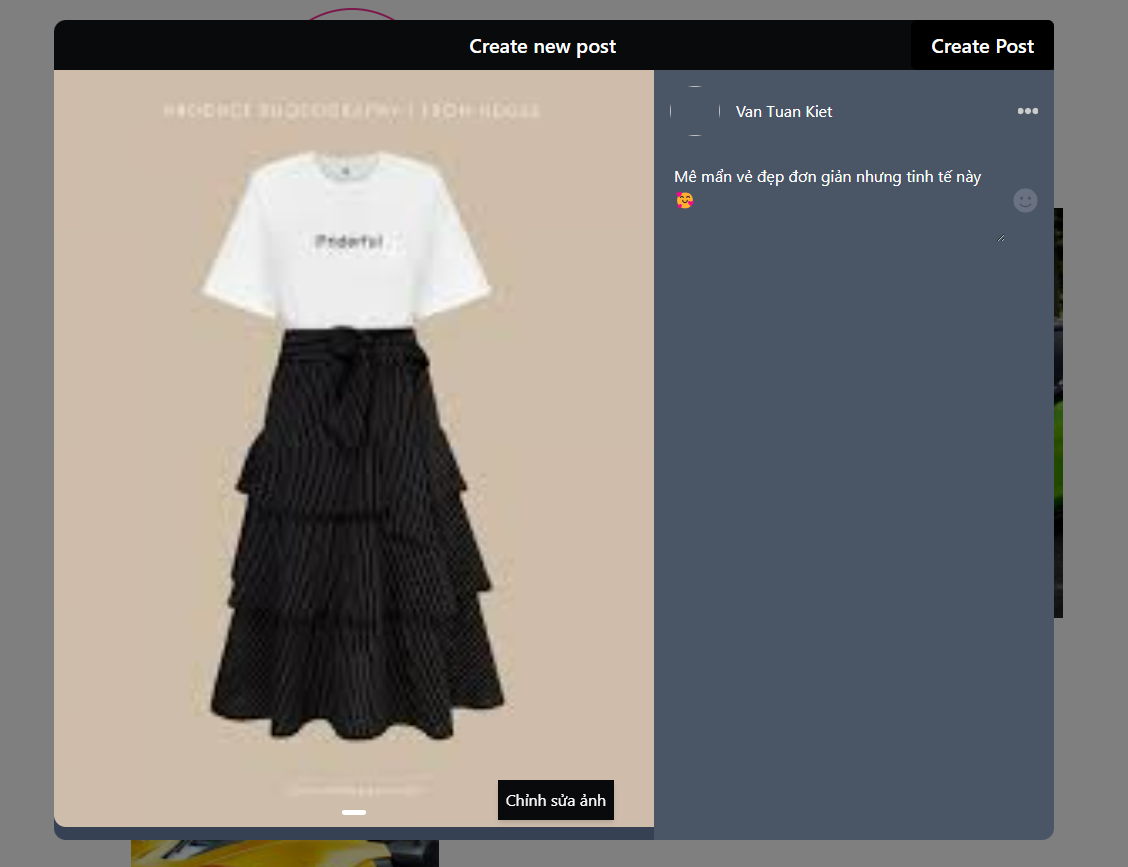
\includegraphics[width=1\textwidth]{img/instagram/bai_viet_hinh_anh.png}
    \caption{Tạo vài viết hình ảnh}
\end{figure}

\FloatBarrier % <-- Dòng này sẽ khóa ảnh phía trên không bị dời xuống



\begin{figure}[H]
    \centering
    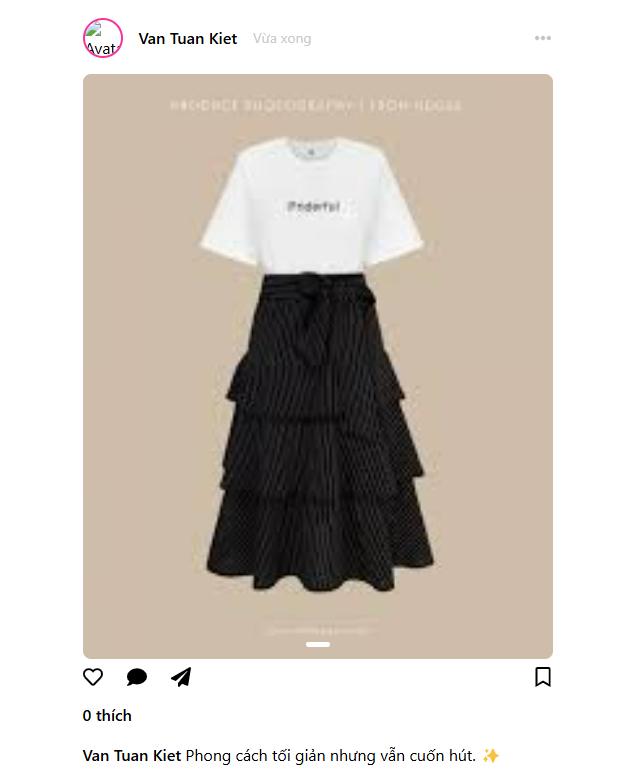
\includegraphics[width=1\textwidth]{img/instagram/bai_viet_hinh_anh_2.png}
    \caption{Kết quả tạo bài viết hình ảnh}
\end{figure}

\FloatBarrier % <-- Dòng này sẽ khóa ảnh phía trên không bị dời xuống

\subsection{Video}

\section{Chức năng tương tác}
\subsection{Like}
\begin{figure}[H]
    \centering
    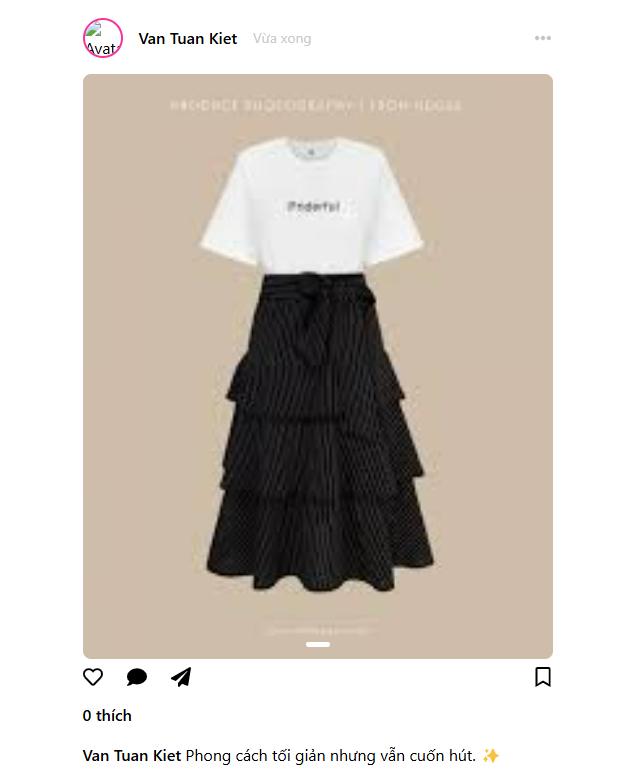
\includegraphics[width=1\textwidth]{img/instagram/bai_viet_hinh_anh_2.png}
    \caption{Ảnh trước like}
\end{figure}

\FloatBarrier % <-- Dòng này sẽ khóa ảnh phía trên không bị dời xuống


\begin{figure}[H]
    \centering
    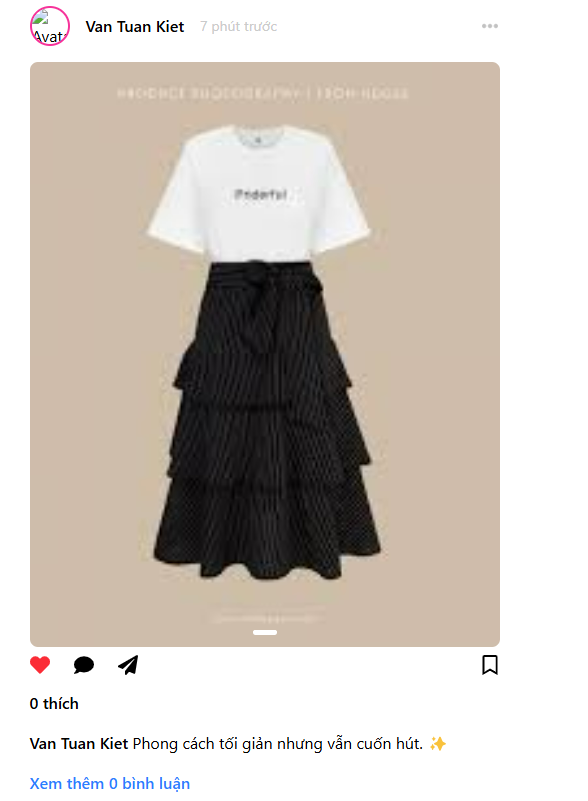
\includegraphics[width=1\textwidth]{img/instagram/like.png}
    \caption{Ảnh sau like}
\end{figure}

\FloatBarrier % <-- Dòng này sẽ khóa ảnh phía trên không bị dời xuống

\subsection{Comment} 
\begin{figure}[H]
    \centering
    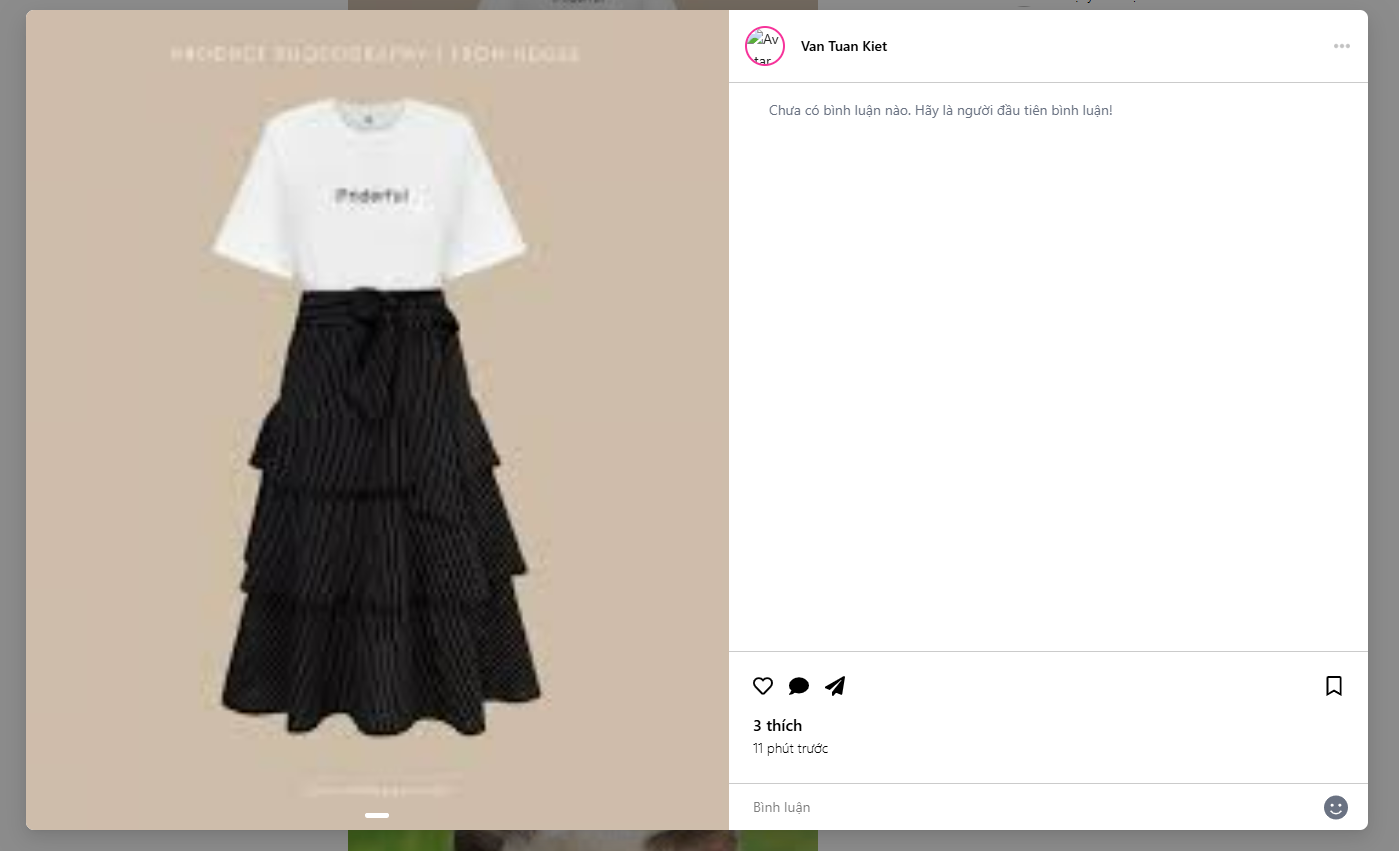
\includegraphics[width=1\textwidth]{img/instagram/chua_binh_luan.png}
    \caption{Ảnh chưa bình luận}
\end{figure}

\FloatBarrier % <-- Dòng này sẽ khóa ảnh phía trên không bị dời xuống

\begin{figure}[H]
    \centering
    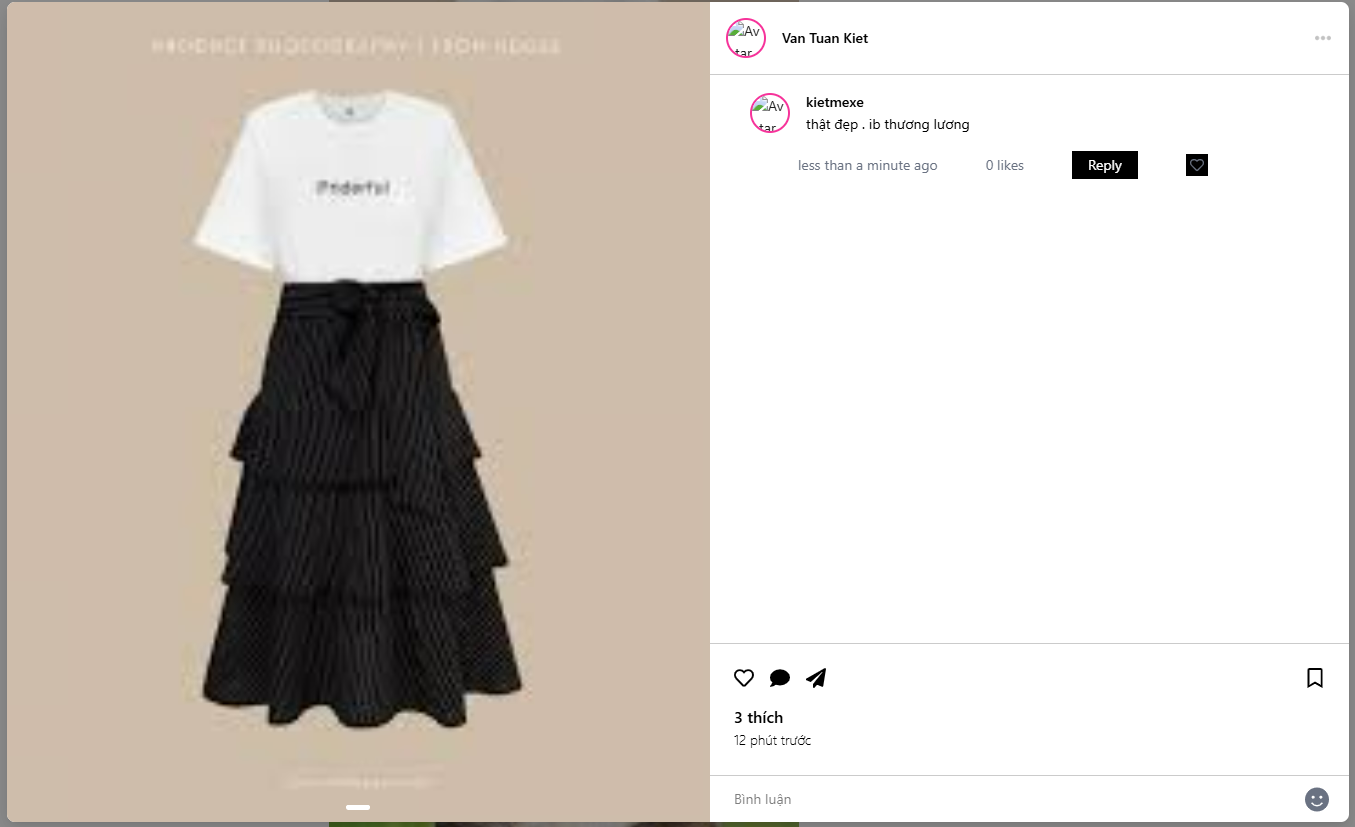
\includegraphics[width=1\textwidth]{img/instagram/da_binh_luan.png}
    \caption{Ảnh đã bình luận}
\end{figure}

\FloatBarrier % <-- Dòng này sẽ khóa ảnh phía trên không bị dời xuống

\section{Chức năng quản lí bạn bè}
\subsection{Thêm bạn}
\begin{figure}[H]
    \centering
    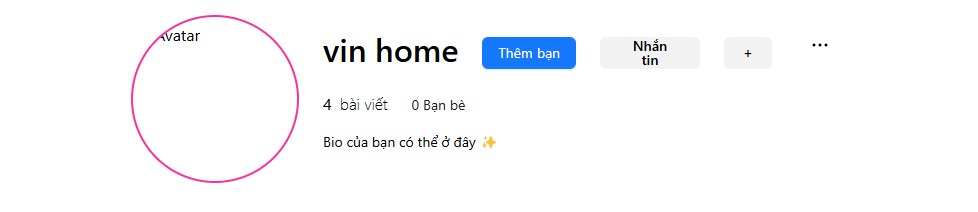
\includegraphics[width=1\textwidth]{img/instagram/them_ban.png}
    \caption{Ảnh thêm bạn}
\end{figure}

\FloatBarrier % <-- Dòng này sẽ khóa ảnh phía trên không bị dời xuống
\begin{figure}[H]
    \centering
    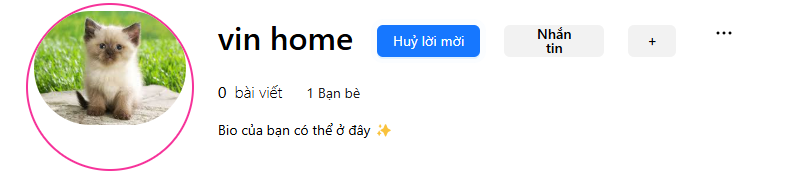
\includegraphics[width=1\textwidth]{img/instagram/huy_loi_moi.png}
    \caption{Ảnh huỷ lời mời}
\end{figure}

\FloatBarrier % <-- Dòng này sẽ khóa ảnh phía trên không bị dời xuống

\begin{figure}[H]
    \centering
    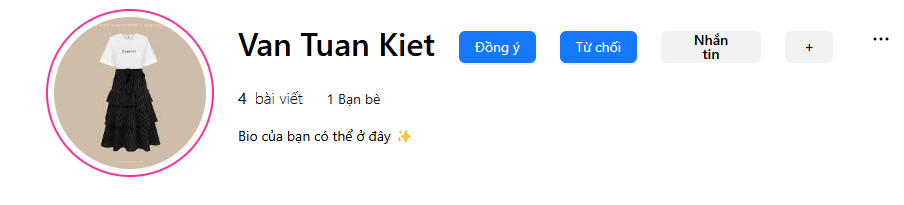
\includegraphics[width=1\textwidth]{img/instagram/chap_nha_tu_choi.png}
    \caption{Ảnh chấp nhận , từ chối lời mời}
\end{figure}

\FloatBarrier % <-- Dòng này sẽ khóa ảnh phía trên không bị dời xuống

\subsection{Huỷ kết bạn}
\begin{figure}[H]
    \centering
    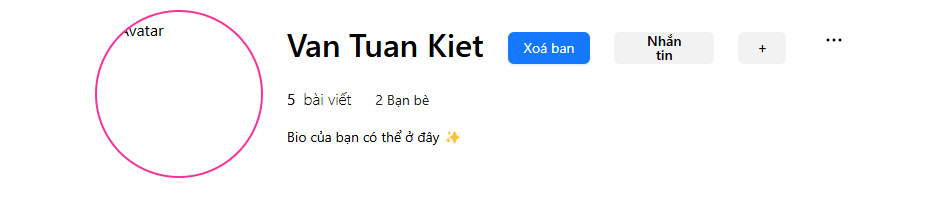
\includegraphics[width=1\textwidth]{img/instagram/xoa_ban.png}
    \caption{Ảnh đã là bạn bè , có thể xoá bạn}
\end{figure}

\FloatBarrier % <-- Dòng này sẽ khóa ảnh phía trên không bị dời xuống

\subsection{Danh sách bạn bè}
\begin{figure}[H]
    \centering
    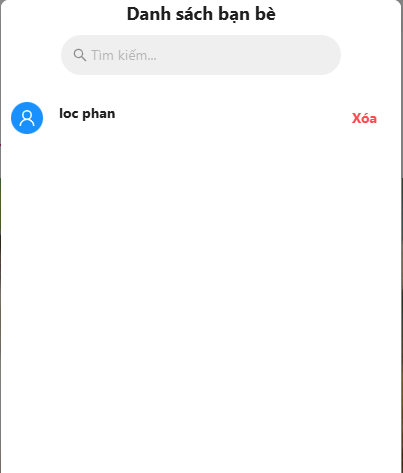
\includegraphics[width=1\textwidth]{img/instagram/danh_sach_ban_be.png}
    \caption{Ảnh danh sách bạn bè}
\end{figure}

\FloatBarrier % <-- Dòng này sẽ khóa ảnh phía trên không bị dời xuống


\section{Chức năng quản lí hồ sơ cá nhân}
\subsection{Cập nhật thông tin người dùng}
\begin{figure}[H]
    \centering
    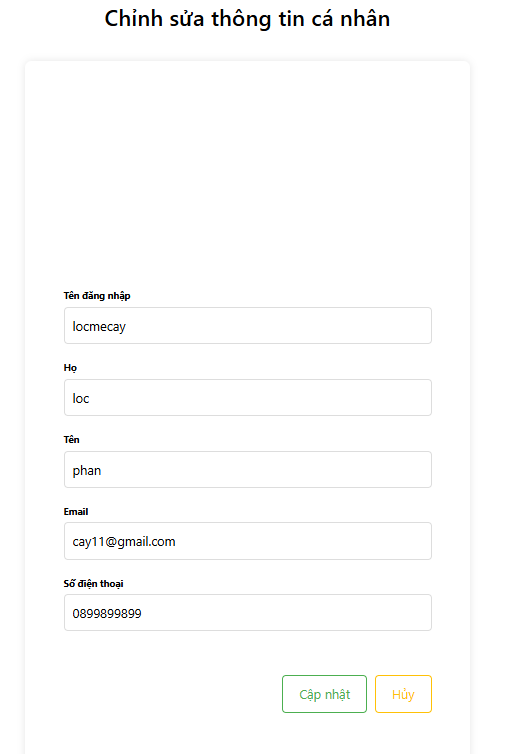
\includegraphics[width=1\textwidth]{img/instagram/đổi tên phan thành hoàng.png}
    \caption{Đổi tên phan thành hoàng}
\end{figure}

\FloatBarrier % <-- Dòng này sẽ khóa ảnh phía trên không bị dời xuống

\begin{figure}[H]
    \centering
    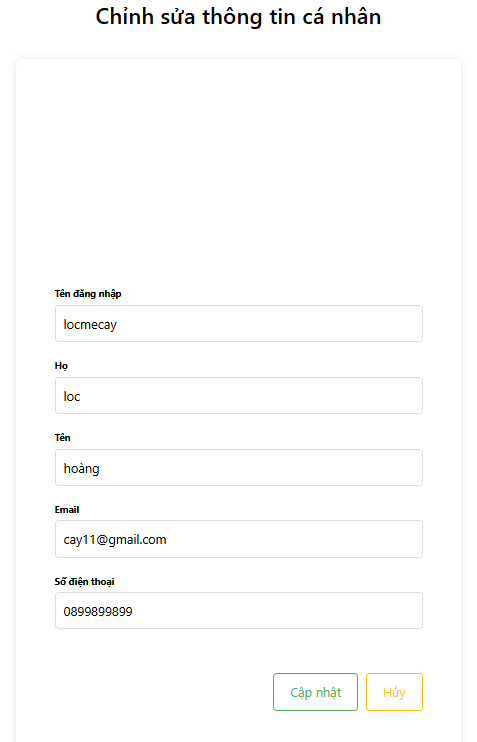
\includegraphics[width=1\textwidth]{img/instagram/kết quả đổi tên.png}
    \caption{Kết quả đổi tên}
\end{figure}

\FloatBarrier % <-- Dòng này sẽ khóa ảnh phía trên không bị dời xuống
\subsection{Cập nhật ảnh đại diện}
\begin{figure}[H]
    \centering
    % 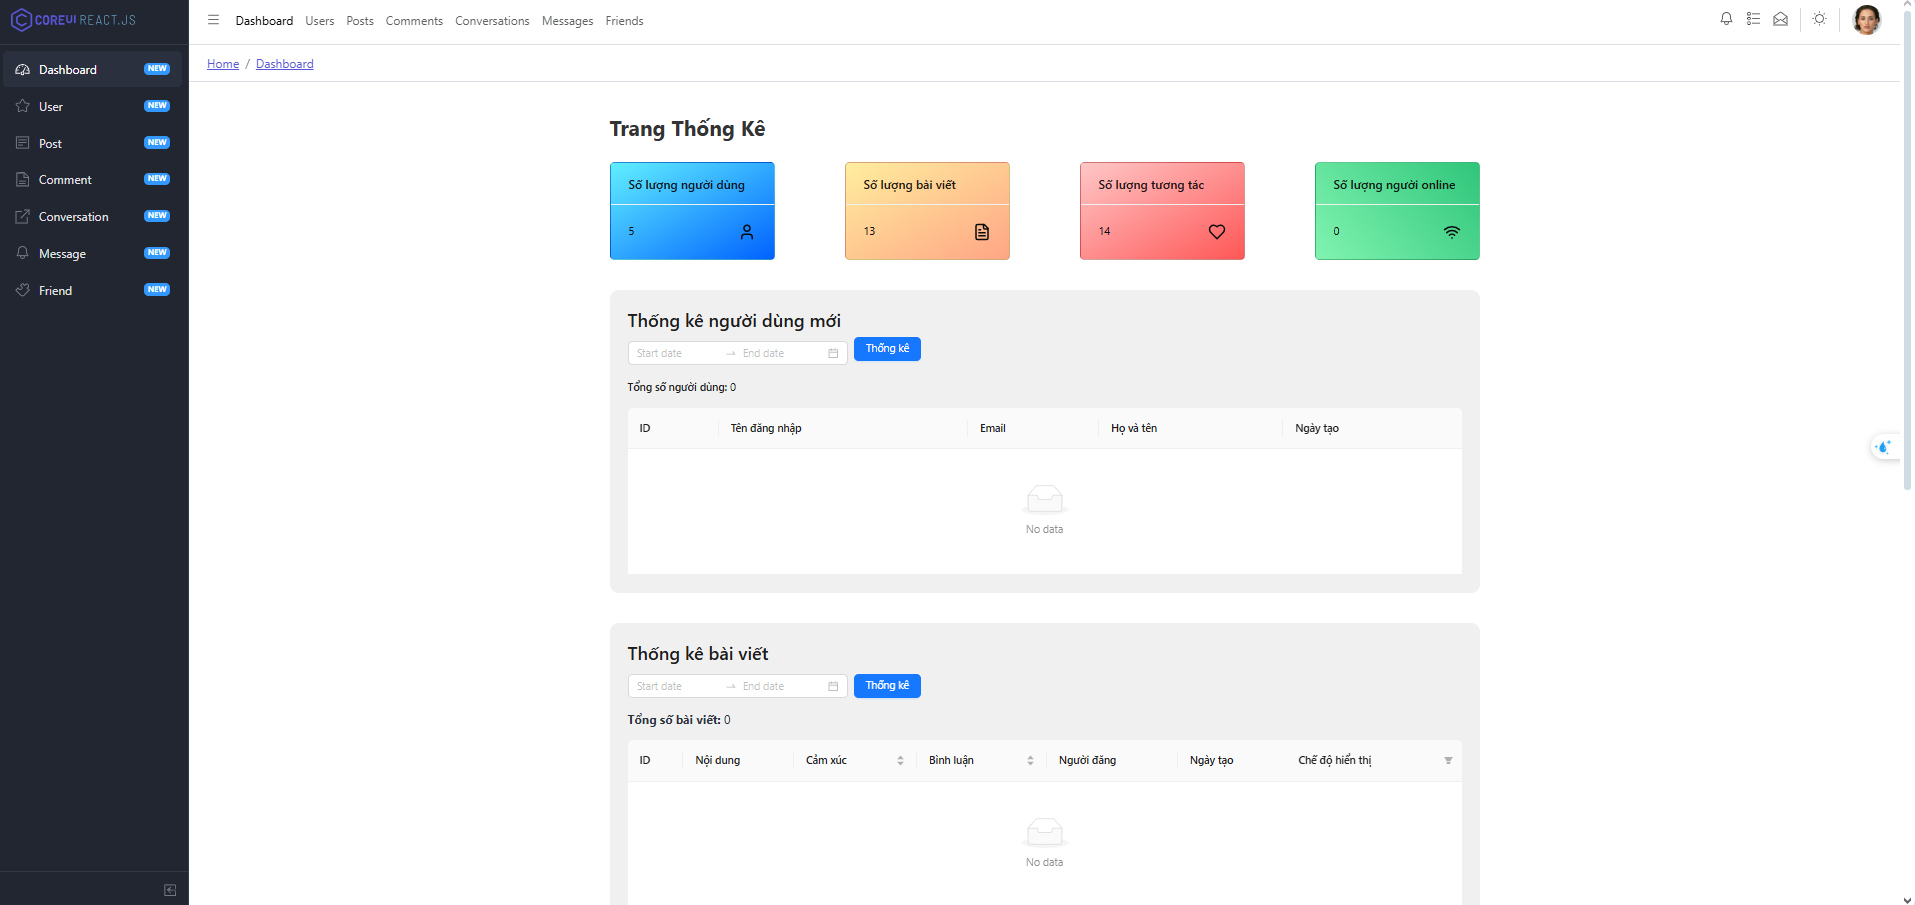
\includegraphics[width=1\textwidth]{img/instagram/trang_admin.png} mở comment và thay link ảnh vô
    \caption{Ảnh trước khi cập nhật}
\end{figure}

\FloatBarrier % <-- Dòng này sẽ khóa ảnh phía trên không bị dời xuống

\begin{figure}[H]
    \centering
    % 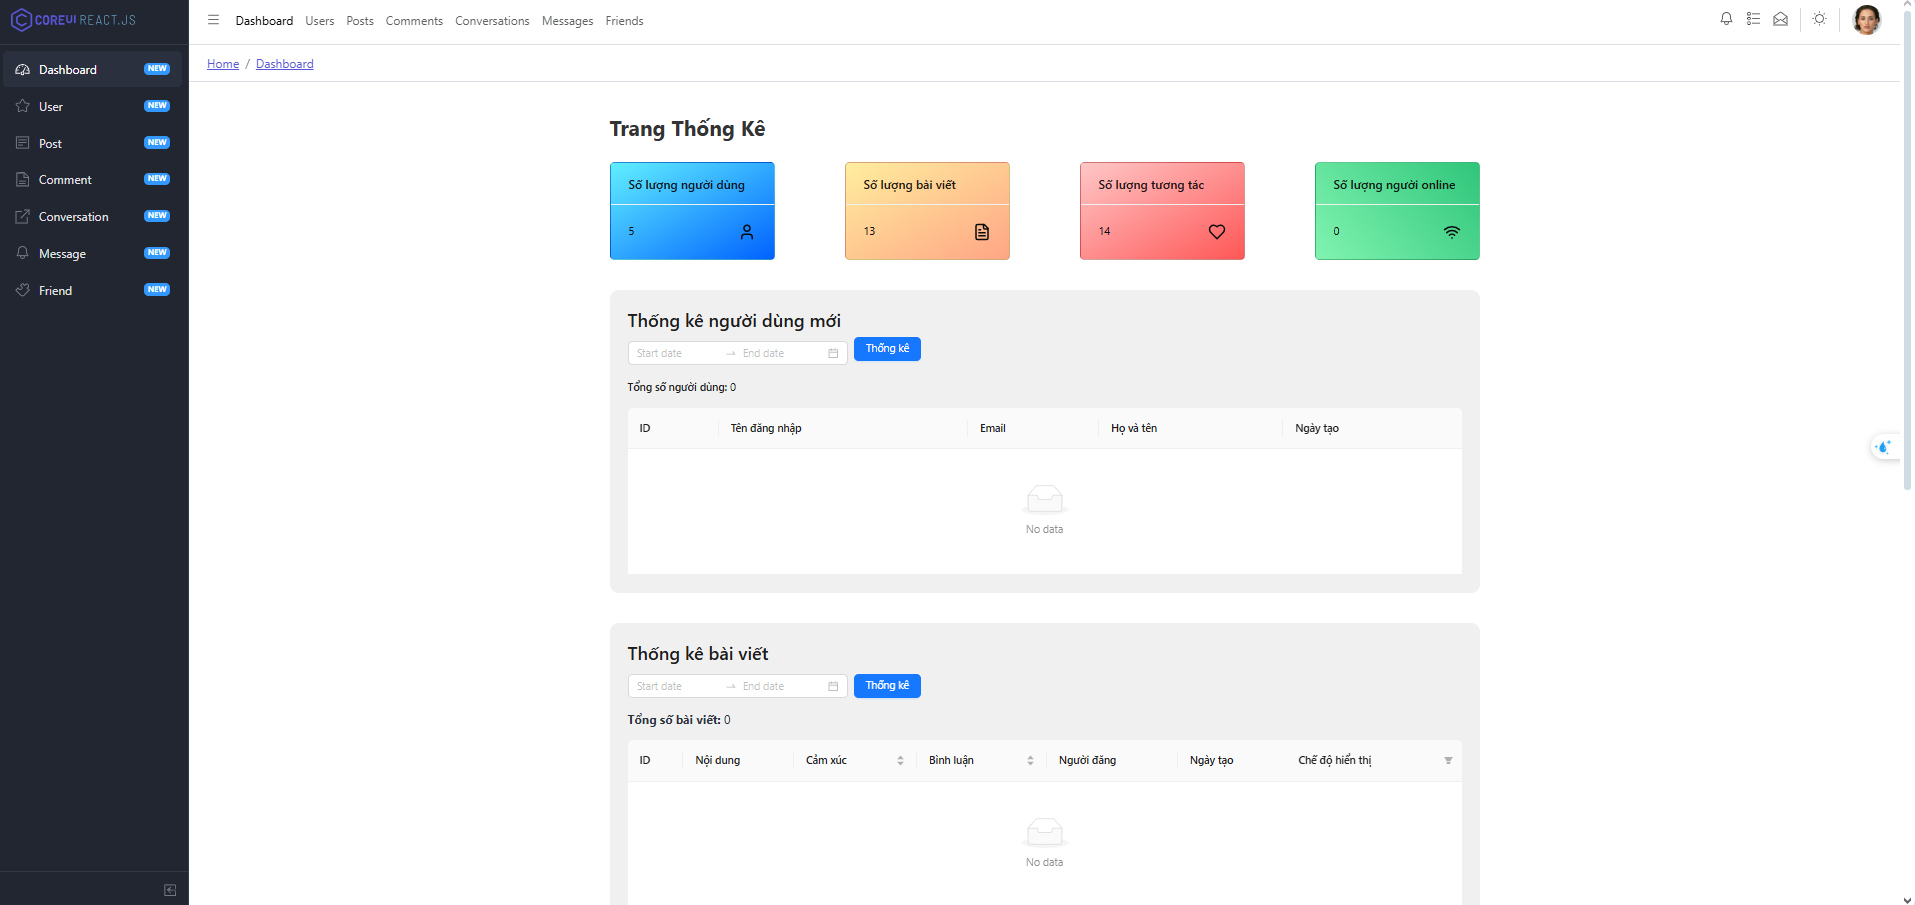
\includegraphics[width=1\textwidth]{img/instagram/trang_admin.png} mở comment và thay link ảnh vô
    \caption{Ảnh sau khi cập nhật}
\end{figure}

\FloatBarrier % <-- Dòng này sẽ khóa ảnh phía trên không bị dời xuống

\section{Trang Admin}
\begin{figure}[H]
    \centering
    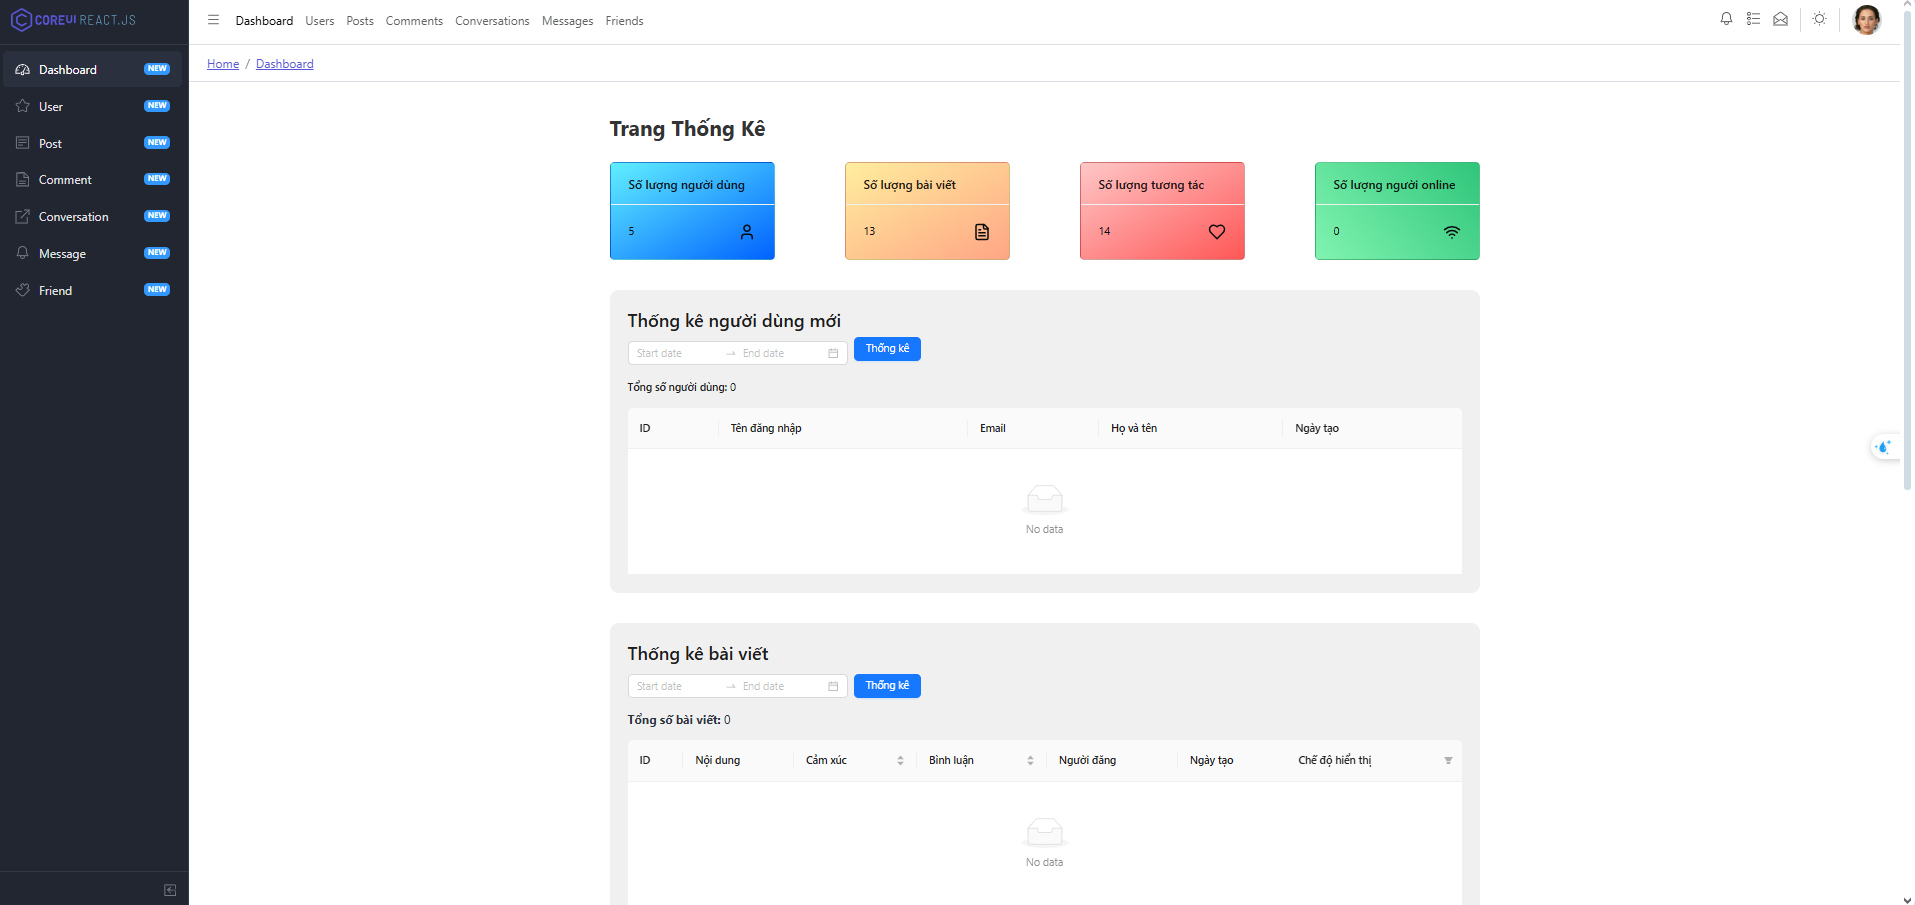
\includegraphics[width=1\textwidth]{img/instagram/trang_admin.png}
    \caption{Ảnh trang admin}
\end{figure}

\FloatBarrier % <-- Dòng này sẽ khóa ảnh phía trên không bị dời xuống
\subsection{quản lí user}
\begin{figure}[H]
    \centering
    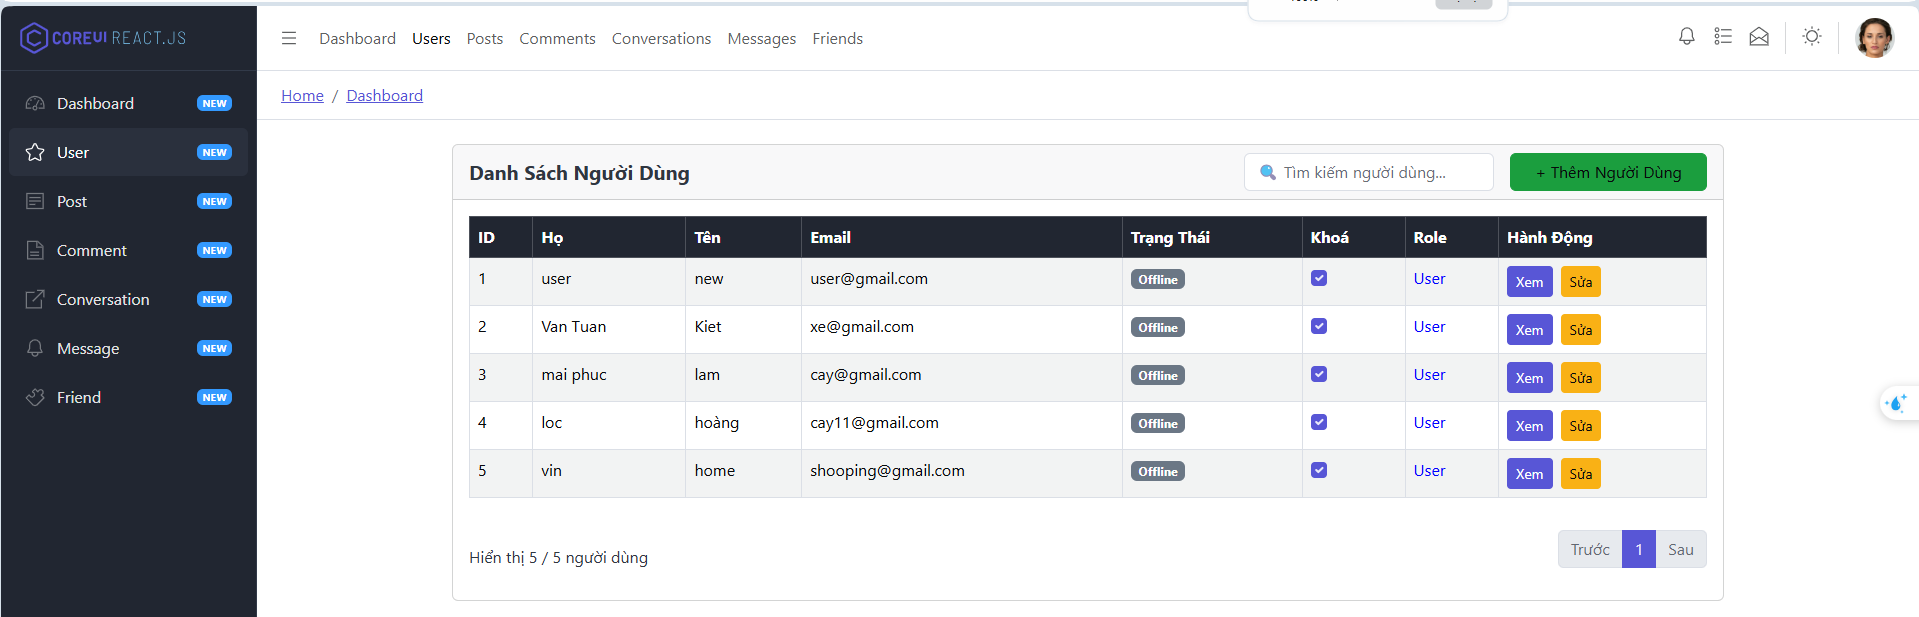
\includegraphics[width=1\textwidth]{img/instagram/trang_quản_lí_user.png}
    \caption{Ảnh trang quản lí user}
\end{figure}

\FloatBarrier % <-- Dòng này sẽ khóa ảnh phía trên không bị dời xuống

\subsection{quản lí post}
\begin{figure}[H]
    \centering
    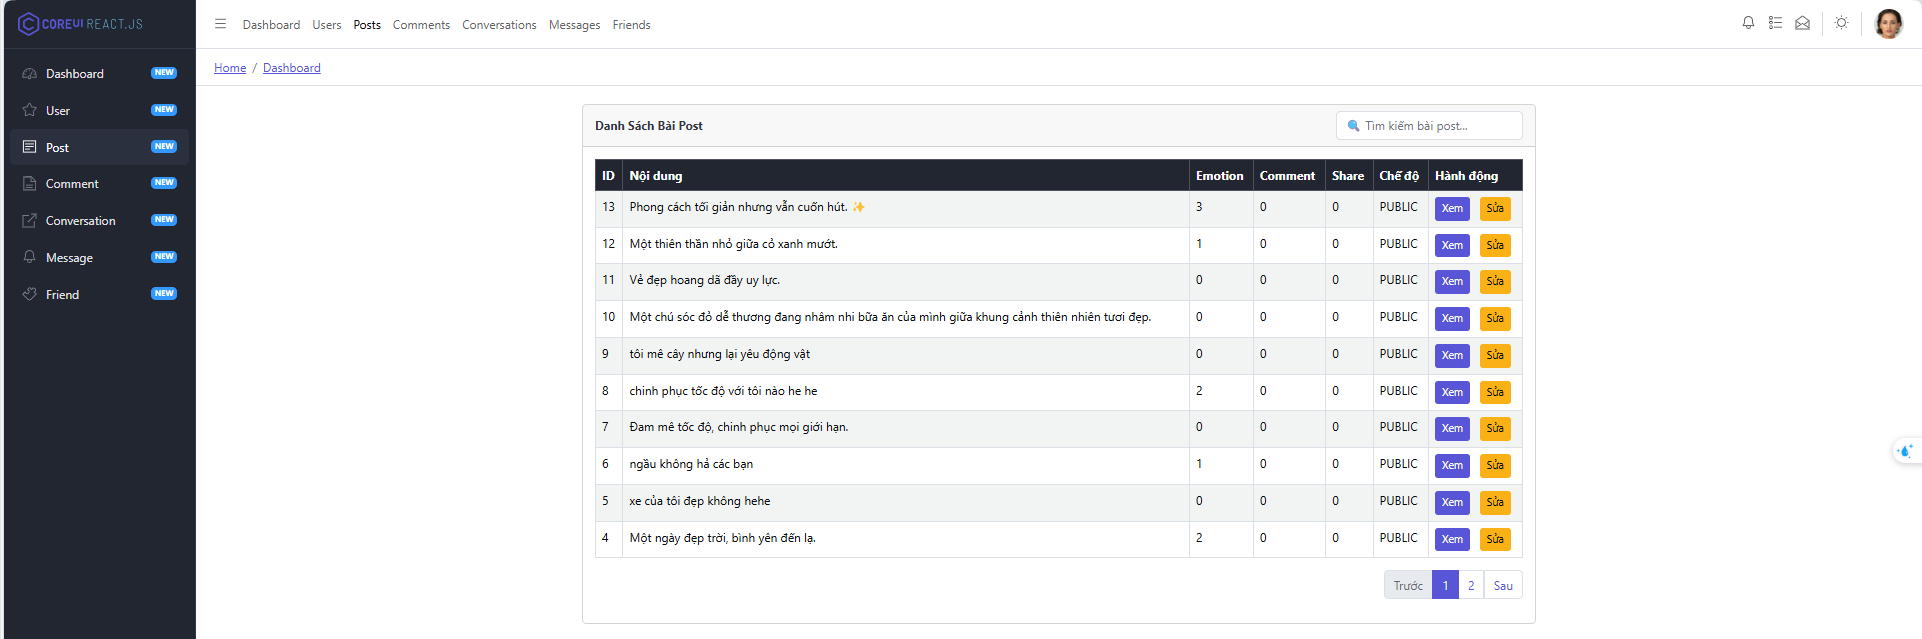
\includegraphics[width=1\textwidth]{img/instagram/trang_quan_li_post.png}
    \caption{Ảnh trang quản lí user}
\end{figure}

\FloatBarrier % <-- Dòng này sẽ khóa ảnh phía trên không bị dời xuống

\section{Nhắn tin real time}
\begin{figure}[H]
    \centering
    \includegraphics[width=1\textwidth]{img/instagram/Nhắn tin real time.png}
    \caption{Ảnh tin nhắn ở người 1}
\end{figure}

\FloatBarrier % <-- Dòng này sẽ khóa ảnh phía trên không bị dời xuống

\begin{figure}[H]
    \centering
    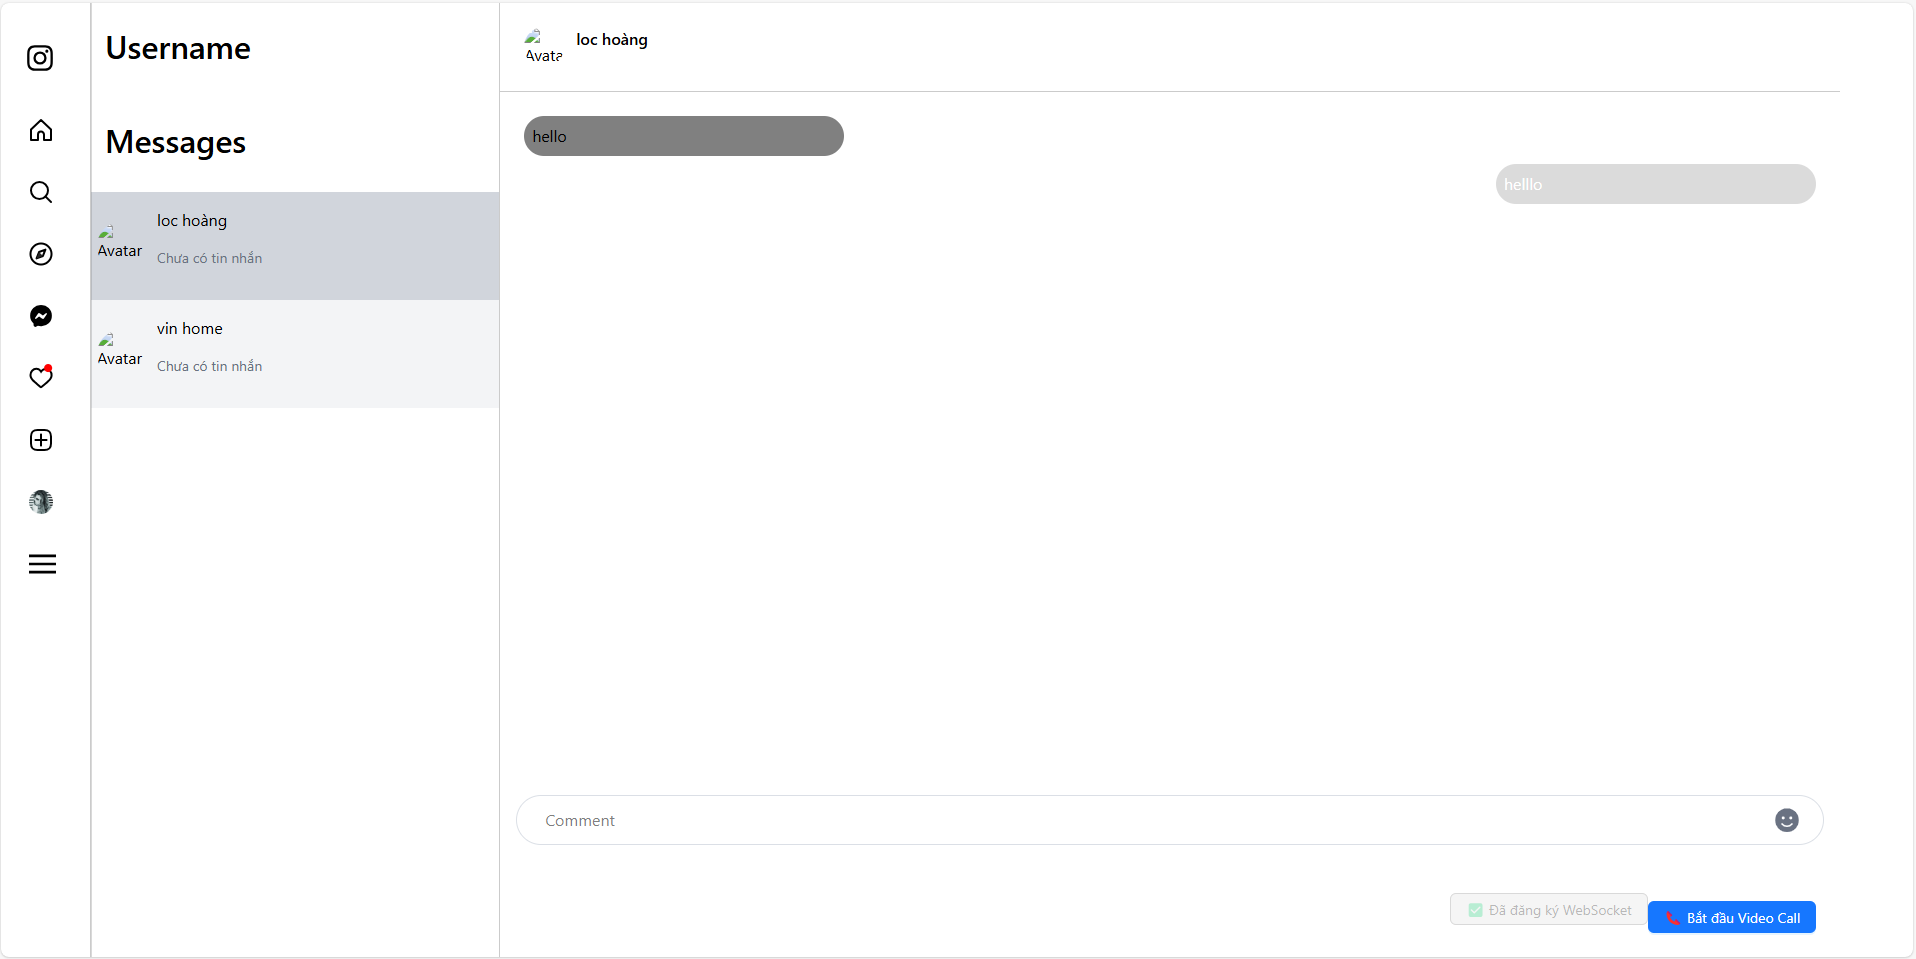
\includegraphics[width=1\textwidth]{img/instagram/nhan_tin_real_time_2.png}
    \caption{Ảnh tin nhắn ở người 2}
\end{figure}

\FloatBarrier % <-- Dòng này sẽ khóa ảnh phía trên không bị dời xuống

\section{Gọi real time}
\begin{figure}[H]
    \centering
    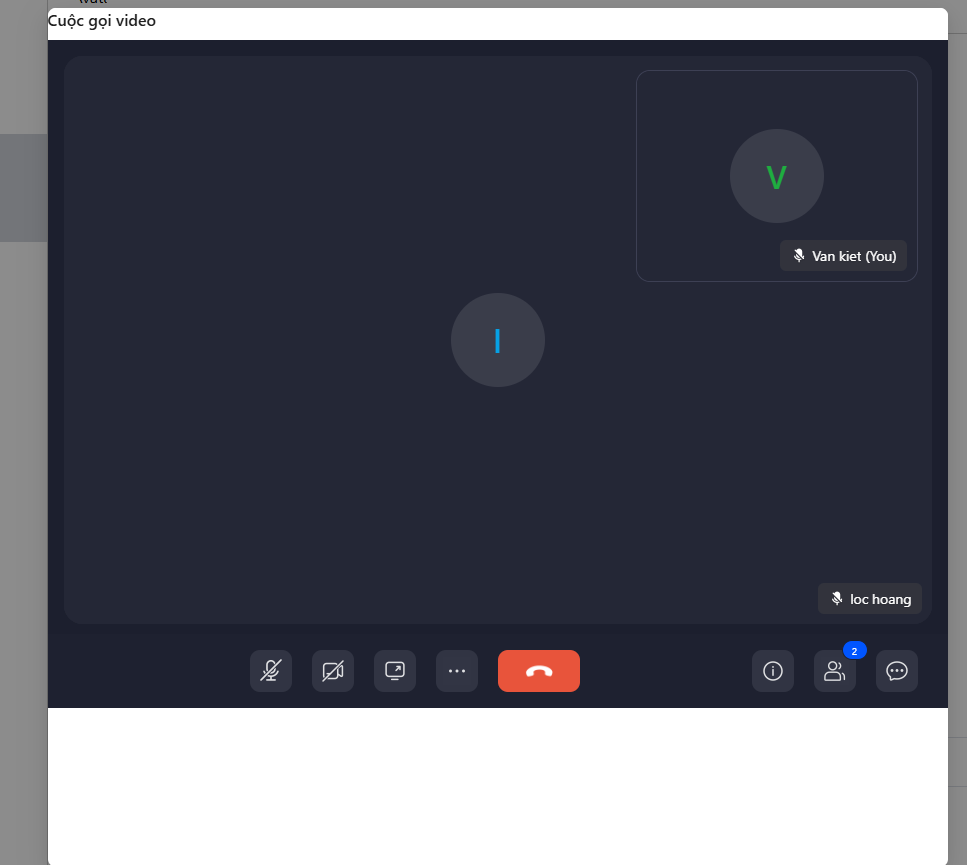
\includegraphics[width=1\textwidth]{img/instagram/ảnh gọi người 1.png}
    \caption{Ảnh gọi real time ở người 1}
\end{figure}

\FloatBarrier % <-- Dòng này sẽ khóa ảnh phía trên không bị dời xuống

\begin{figure}[H]
    \centering
    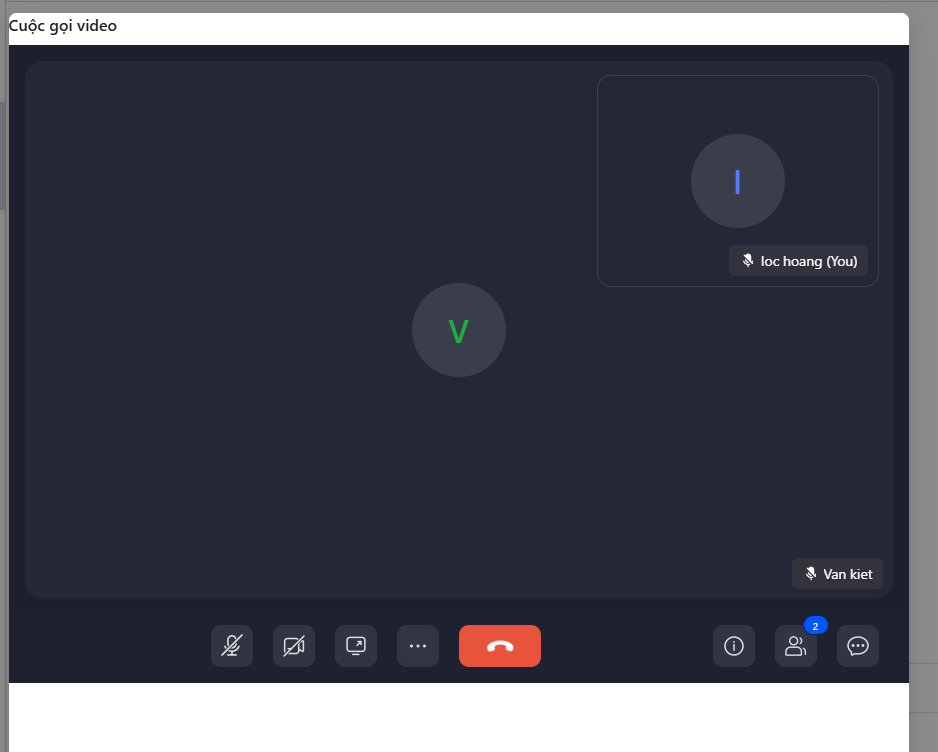
\includegraphics[width=1\textwidth]{img/instagram/ảnh gọi người 2.png}
    \caption{Ảnh gọi real time ở người 2}
\end{figure}

\FloatBarrier % <-- Dòng này sẽ khóa ảnh phía trên không bị dời xuống

\section{Thông báo rael time}
\begin{figure}[H]
    \centering
    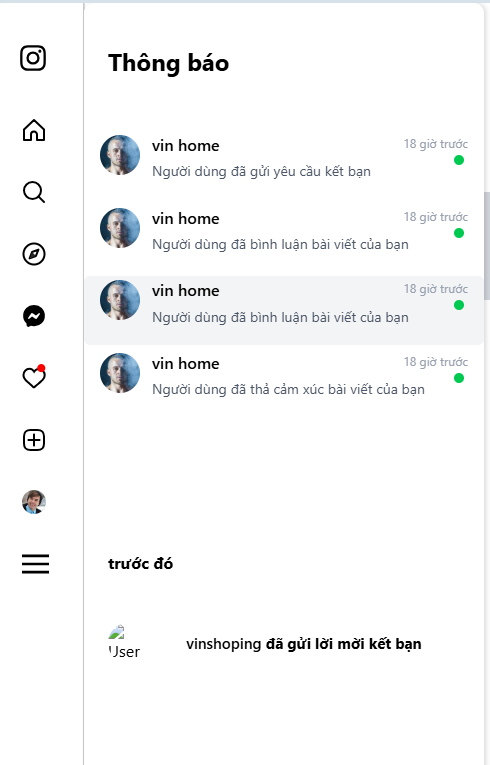
\includegraphics[width=1\textwidth]{img/instagram/có thông báo .png}
    \caption{Ảnh thông báo khi có người bình luận , gửi kết bạn}
\end{figure}

\FloatBarrier % <-- Dòng này sẽ khóa ảnh phía trên không bị dời xuống
